\section{Wakeflow: A Python Package For Semi-Analytic Models of Planet Wakes}

\section{Wake Formation}

\subsection{The Shearing Sheet Approximation}

\section{Wake Propagation}

\subsection{Power Law Disks}

\subsection{Velocity Perturbations}

From \citet{rafikov2002a}, the conservation of the Riemann invariant $R_+$ gives for the radial Velocity
\begin{align}
    u = 2\frac{c_0-c}{\gamma -1}=-2\frac{c_0}{\gamma + 1}\psi,
\end{align}
where we define $\psi$ as
\begin{align}
    \psi = \frac{\gamma+1}{\gamma-1} \frac{c - c_0}{c_0},
\end{align}
which is the sound speed perturbation with a constant scale factor. Following \citet{rafikov2002a}, we then derive an expression for $\psi$ in terms of the density perturbation $\chi$ by assuming that the gas obeys a locally polytropic equation of state given by 
\begin{align}
    P = P_0(r) \left[ \frac{\Sigma}{\Sigma_0(r)} \right]^\gamma. \label{eq:poly_EOS}
\end{align}
The sound speed is then
\begin{align}
    c^2 = \frac{\partial P}{\partial \Sigma} = c_0^2(r) \left[ \frac{\Sigma}{\Sigma_0(r)} \right]^{\gamma-1}.
\end{align}
\citet{rafikov2002a} then finds a relation between the density and sound speed perturbations, accurate to second order in $\psi$, found by expanding the above expression. This yields
\begin{align}
    \frac{\Sigma - \Sigma_0}{\Sigma_0} = \frac{2}{\gamma + 1}\psi + \frac{3 - \gamma}{\left( \gamma + 1  \right)^2} \psi^2 + \mathcal{O}(\psi^3). \label{eq:psi_exp}
\end{align}
Taking this expression to first order only, we write $u$ in terms of the density perturbation, and then in terms of $\chi$ by substituting Equation \feqr. 
\begin{align}
    u = - c_0 \frac{\Sigma - \Sigma_0}{\Sigma_0} = -2 \frac{c_0}{\gamma + 1} \frac{\chi}{g(r)}. \label{eq:ap_rad_vel}
\end{align}
Similarly, \citet{rafikov2002a} finds the azimuthal velocity as
\begin{align}
    v \approx -2 \frac{c_0^2}{\Delta\Omega r} \frac{1}{\gamma + 1} \psi,
\end{align}
giving to first order in $\psi$
\begin{align}
    v \approx - \frac{c_0^2}{\Delta \Omega r} \frac{\Sigma - \Sigma_0}{\Sigma_0} = - \frac{2}{\gamma + 1} \frac{c_0^2}{\Delta \Omega r} \frac{\chi}{g(r)}. \label{eq:ap_az_vel}
\end{align}
Equations \ref{eq:ap_rad_vel} and \ref{eq:ap_az_vel} are the expressions used in \citet{bollati2021} to calculate the velocity perturbations in the non-linear regime. Since these are only accurate to first order in $\psi$, the assumption is made that $\psi \ll 1$; indeed \citet{bollati2021} notes that terms proportional to $\psi^2$ are discarded in the derivation of the Burgers evolution \feqr, and thus also in the calculation of $\chi$ from which $u$ and $v$ are calculated. However it is not clear that neglecting the most non-linear terms to calculate the density perturbation $\chi$ necissitates the truncation of the equation of state in the same way. Since we are in particular interested in the velocity perturbations, and in planet masses comparable to the thermal mass, we should check if the assumption that $\psi \ll 1$ holds.

Rearranging Equation \ref{eq:poly_EOS} for $\psi$ we find
\begin{align}
    \psi = \frac{\gamma + 1}{\gamma - 1} \left[ \left( \frac{\Sigma-\Sigma_0}{\Sigma_0} +1  \right)^{\psi-1/2} -1 \right],
\end{align}
which can be written equivalently in terms of $\chi$ using Equation \feqr giving
\begin{align}
    \boxed{\psi = \frac{\gamma + 1}{\gamma - 1} \left[ \left( \frac{2}{\gamma + 1} \frac{\chi}{g(r)} +1  \right)^{\psi-1/2} -1 \right]}. \label{eq:psi_exact}
\end{align}
Equation \ref{eq:psi_exact} is an \textit{exact} relation between $\chi$ and $\psi$, which we will use to check the aforementioned assumption that $\psi<1$ in the non-linear regime solution. We construct three dimensionless \textsc{wakeflow} models, with embedded planet masses of $0.5, 1.0$ and $2.0 \, M_{\rm{th}}$ respectively, all placed in orbit around a $1 \, M_{\rm{\odot}}$ star at an orbital radius of $r=1$. For all models, we choose $p=2.25$ and $q=0.25$ such that $\Sigma \propto r^{-1}$, and an aspect ratio $H/r=0.1$ at $r=1$. Figure \ref{fig:psi_comparison} shows the values of $\psi$ for each of these models, and demonstrates that even for the lowest planet mass model the value of $\psi$ nearby the planet is as large as $\sim \hspace{-0.23em} 0.6$ and so the second order terms will clearly be important even in this case. For masses $\ge \hspace{-0.23em} M_\mathrm{th}$ the problem is even worse, as there are regions where $\psi \gtrsim 1$ causing the expansion given in Equation \ref{eq:psi_exp} to diverge.

\begin{figure}[H]
    \centering
    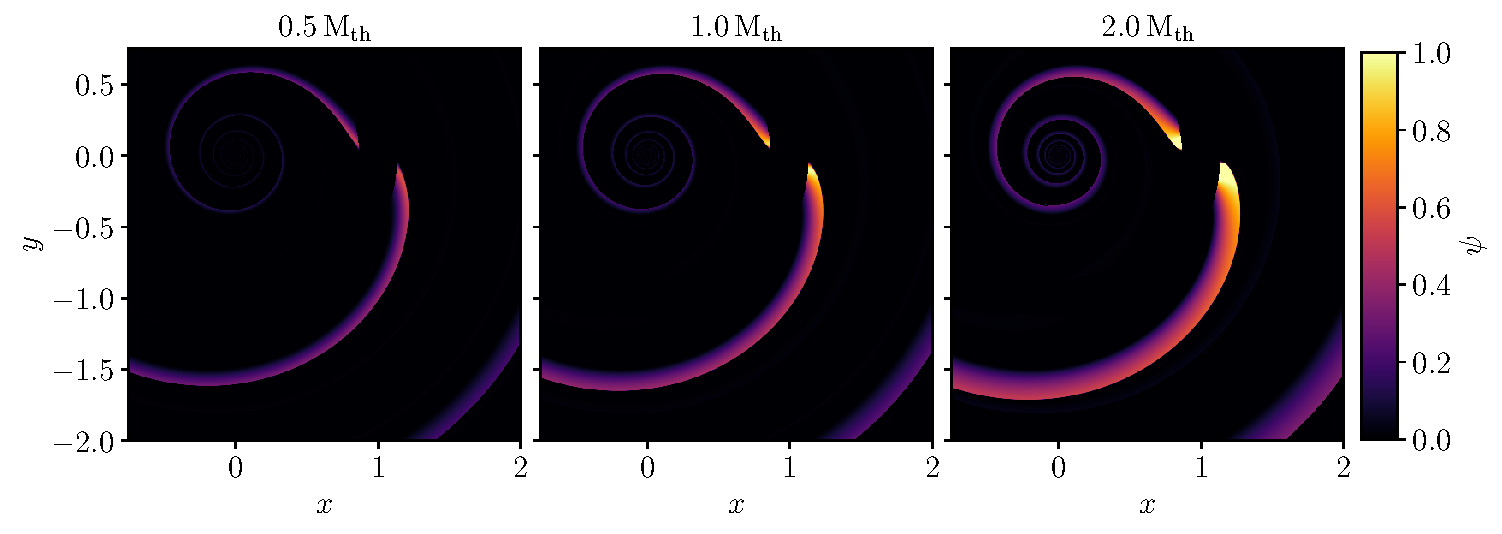
\includegraphics[width = 0.95\textwidth]{figures/psi 2.pdf}
    \caption{Comparison of the values of $\psi$ calculated from Equation \ref{eq:psi_exact} for three \textsc{wakeflow} models with planet masses of $0.5, 1.0$ and $2.0 \, M_{\rm{th}}$ respectively. Clearly one cannot assume that $\psi \ll 1$ even for the lowest mass model, expecially nearby the planet. For the two larger masses, there are even regions where $\psi > 1$.}
    \label{fig:psi_comparison}
\end{figure}

\begin{figure}[H]
    \centering
    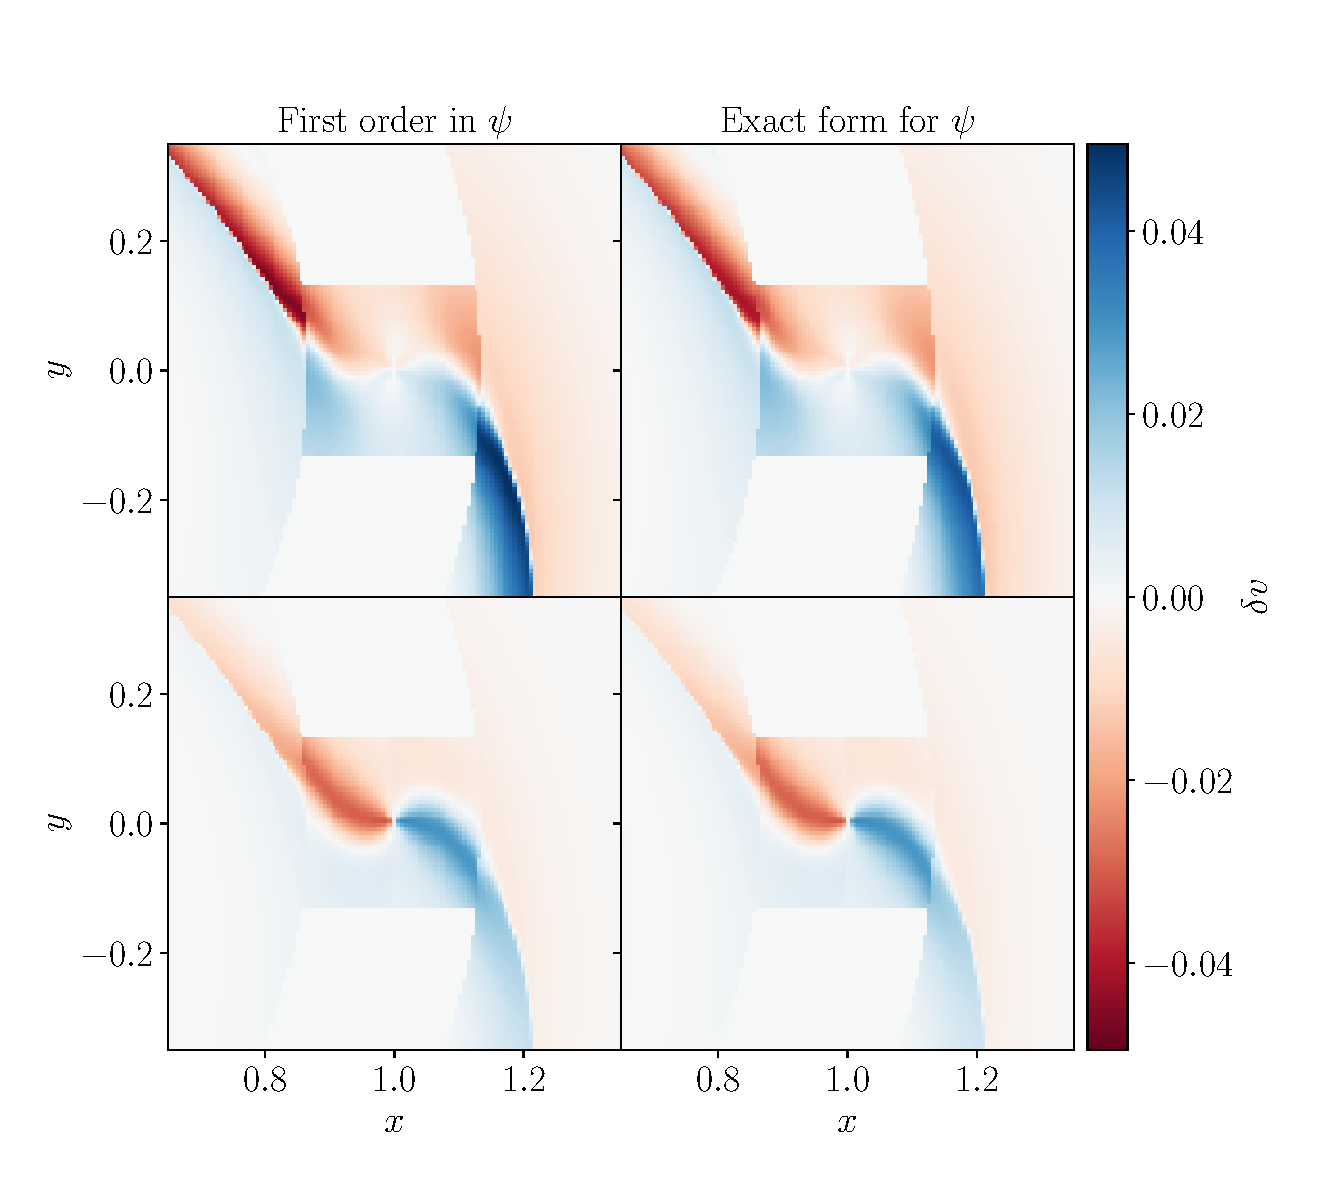
\includegraphics[width = 0.65\textwidth]{figures/0_5_mth.pdf}
    \caption{}
    \label{fig:0_5mth}
\end{figure}

\begin{figure}[H]
    \centering
    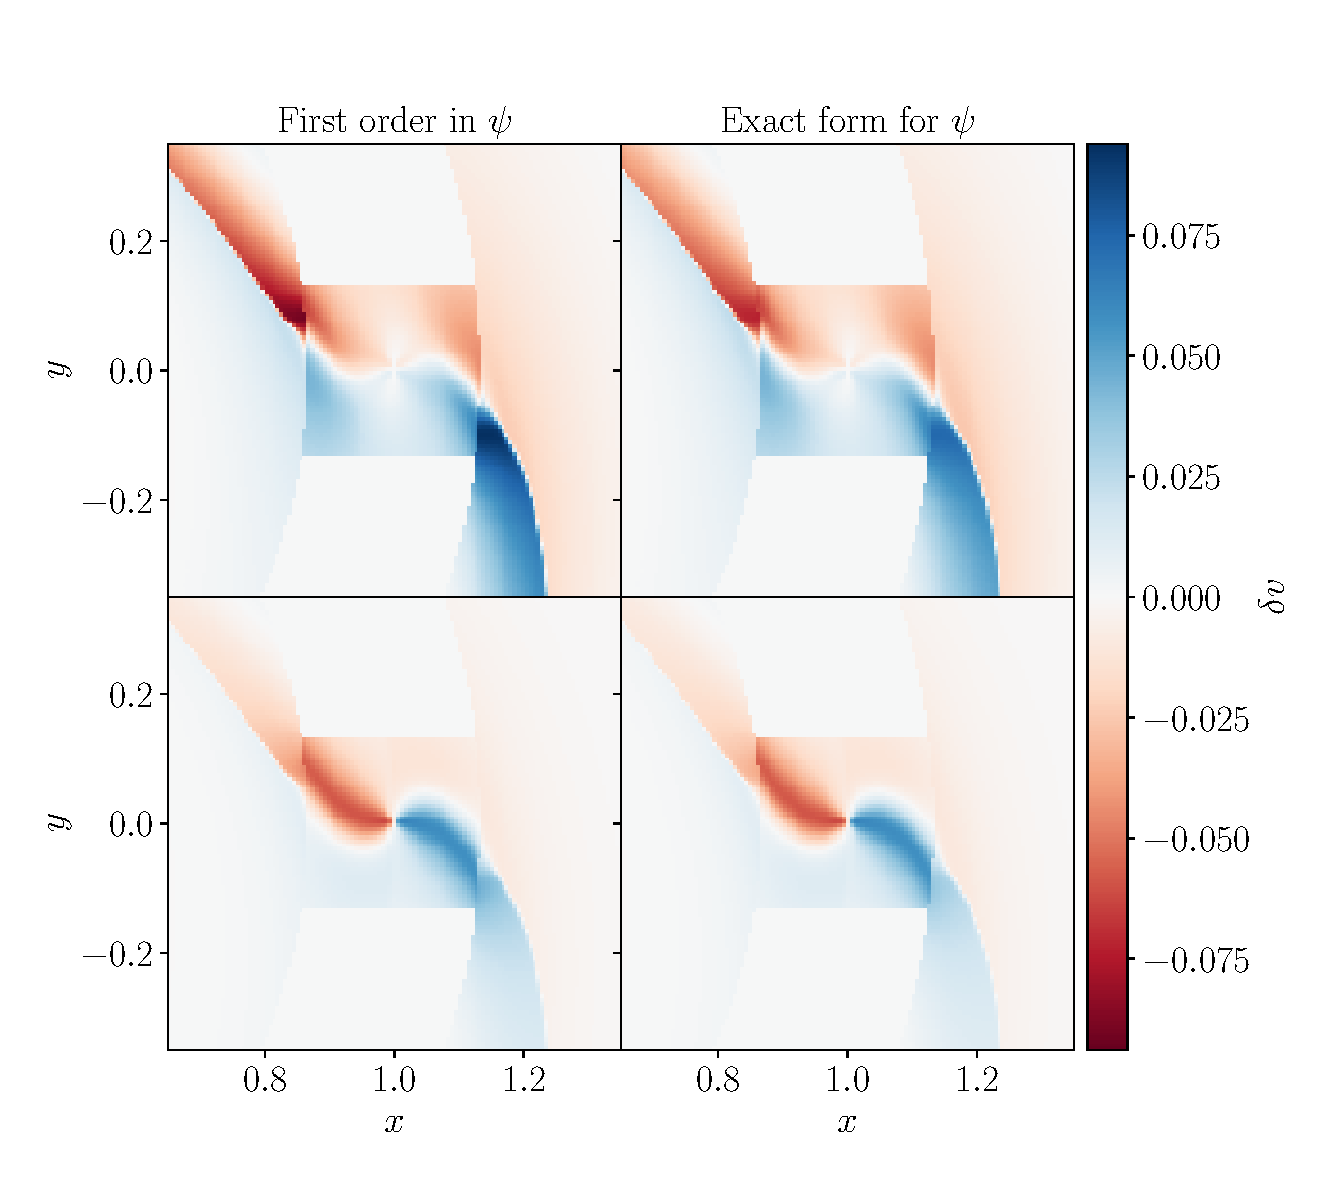
\includegraphics[width = 0.65\textwidth]{figures/1_0_mth.pdf}
    \caption{}
    \label{fig:1_0mth}
\end{figure}

\begin{figure}[H]
    \centering
    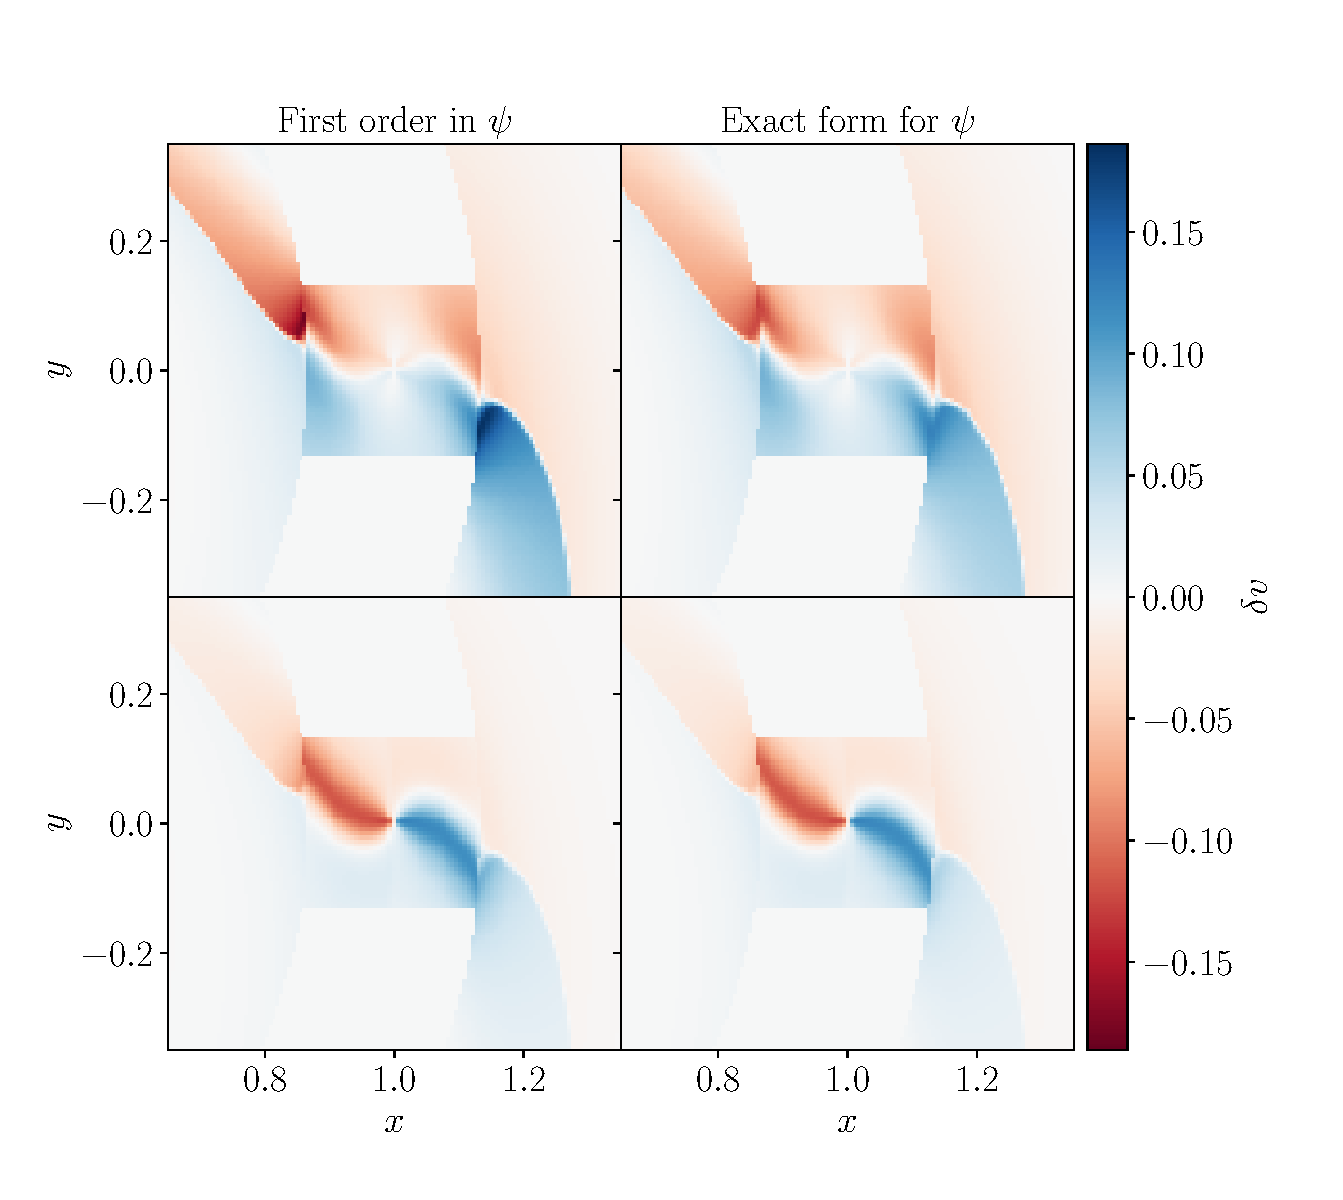
\includegraphics[width = 0.65\textwidth]{figures/2_0_mth.pdf}
    \caption{}
    \label{fig:2_0mth}
\end{figure}

\section{Synthetic Kinematic Observations}

\subsection{Predictions from 2D Models}

\subsection{3D Models}

\subsection{Radiation Transfer}